\chapter{Detailed System Design}


\section{Operator}

\section{EEG Data Acquisition}

\subsection{Module Initialization}

The initialization of the data acquisition module follows the procedure that is 
described in detail in chapter \textit{System Initialization} in the BCI2000 
Project Outline. 

\subsection{System Termination}

The following system termination procedure ensures a graceful shutdown, i.e., 
information cycles through the system one last time and then each module 
terminates. The specific procedure is as follows:

\begin{enumerate}
 \item{Operator sends the system command "Reset" to the EEG Source}
 \item{EEG Source leaves MainDataAcqLoop, and sends the system command "Reset" to Signal Processing}
 \item{When Signal Processing receives "Reset," it terminates its Receiving Thread and sends "Reset" to the Application}
 \item{When the Application receives "Reset," it terminates its Receiving Thread and sends "Reset" to the EEG Source}
 \item{When the EEG Source received "Reset" from the Application, it terminates its Receiving Thread and sends "Reset" to the Operator}
 \item{When the Operator finally receives "Reset," it closes connections to all three core modules}
 \item{Each core module detects the dropped connection to the Operator, then closes all connections and terminates}
\end{enumerate}

\subsubsection{General Principle}

Summarized, the module publishes its requests for parameters and states to the 
Operator module, which configures those and sends them back. After Data 
Acquisition received all parameters and states, it tries to connect to Signal 
Processing and - upon successful connection - sends a positive status message to 
the Operator. After the Operator received status messages from all three core 
modules, the system is fully initialized and is triggered to start, as soon as 
the Operator sends the state \textit{Running} with a value of 1 to the Data 
Acquisition.

\subsubsection{Specific Implementation}

\textit{By May 2003, much of the following detailed description has become
obsolete, mainly by the introduction of a more thorough and unifying
inheritance scheme;} \texttt{GenericADC} \textit{now inherits from}
\texttt{GenericFilter}; \textit{all arguments that referred to global objects
of types} \texttt{PARAMLIST, STATELIST, STATEVECTOR,} \textit{and}
\texttt{CORECOMM} \textit{have been removed in favor of
accessor functions which are part of a new mix-in base class,}
\texttt{Environment}. \textit{A strict privatization of data members and introduction
of accessor functions, as well as a consequent distinction between private,
public, and protected members has taken place, resulting in a minimal set
of details being exposed to code outside the framework itself, which is
still changing, but without consequences for existing ADC and filter code.
From this point of view, updating the following section in detail seemed
problematic. For detailed up-to-date reference, the reader is pointed to the
source code itself. To indicate the most important changes, footnotes have
been added to the existing text which remains unchanged.--jm}\\[1ex]
The system instantiates a new object from a class derived from 
\textit{GenericADC} (details in \ref{class_model_dataacqu}) and passes an empty 
parameter and state list. The constructor for this class fills these empty lists 
with the parameters and states it wants to request from the operator. After the 
operator filled these requests with meaningful values and after state 
\textit{Running} switched to 1, the software enters the main data acquisition 
loop, as below (in pseude code) - adc is a pointer to the derived (from 
GenericADC) object:

\begin{verbatim}
void TfMain::MainDataAcqLoop()
{
 // construct a new GenericDataStore object
 gds=new GenericDataStorage(&paramlist, CoreSocket, SignalProcessingSocket);

 adc->ADInit();

 while state 'Running' is 1
  {
  adc->ADReadDataBlock();

  UpdateStateVector();
  gds->Write2SignalProc(adc->signal, statevector);
  tds->Write2Disk(adc->signal);

  vis->Send2Operator(adc->signal);
  }

 adc->ADShutdown();
}
\end{verbatim}

ADInit() initializes (i.e., configures and starts) the data acquisition process. 
ADReadDataBlock() acquires a data block (\textit{SoftwareCh} channels and 
\textit{SampleBlockSize} samples) with sampling rate \textit{SamplingRate}. 
ADReadDataBlock() DOES NOT return, until the data acquisition for said data 
block has not finished. Finally, ADShutdown() stops the data acquisition upon
exiting the main loop.\footnote{
The \texttt{GenericADC} class now inherits the unified class interface declared
by \texttt{GenericFilter}, which is discussed in section~\ref{class_model}.
The previous \texttt{GenericADC} member functions have been mapped as follows:
\texttt{ADInit()}$\rightarrow$\texttt{Initialize()} -- \texttt{ADReadDataBlock()}$\rightarrow$\texttt{Process()} -- \texttt{ADShutdown()}$\rightarrow$\texttt{Halt()}.
}


\subsection{Implementing Your Own Data Acquisition}

Integrating a new data acquisition board into the system is simple:\footnote{
       The instantiation scheme has been changed to avoid copying and editing
       of framework code (which made it difficult to maintain). Now, you add a line
       \texttt{RegisterFilter(MyADC, 1);} to your ADCs own cpp file, and
       don't touch \texttt{UMain.cpp}.}

\begin{enumerate}
 \item{Derive a class from \textit{GenericADC} in a separate file}
 \item{Implement the constructor and the methods ADInit(), ADReadDataBlock(),
       and ADShutdown() (use the implementations in RandomNumberADC 
       as an example to start with and make sure that your methods
       have the same return values)}
 \item{Include your new unit in the EEGsource project and include 
       its header file in UMain.cpp}
 \item{In UMain.cpp, in \begin{verbatim}TfMain::StartupDataAcquisition()\end{verbatim}
       change the instantiation
       \begin{verbatim}adc=new RandomNumberADC(&paramlist, &statelist);\end{verbatim}}
 \item{Change the type declaration \begin{verbatim}RandomNumberADC *adc;\end{verbatim} 
       in UMain.h to the name of your derived class}  
\end{enumerate}


\subsection{Class Model}
\label{class_model_dataacqu}

This section describes the main classes used for data acquisition. In addition, 
you'll find comments and examples throughout.

\begin{verbatim}
class GenericADC
{
protected:
        int     samplerate;
public:
        GenericADC::GenericADC();
        GenericADC::~GenericADC();
        GenericIntSignal *signal;
        int     ADInit();
        int     ADReadDataBlock();
        int     ADShutdown();
        int     GetSampleRate();
};
\end{verbatim}

One example of an implementation of a derived class from GenericADC is 
RandomNumberADC.

\begin{verbatim}
class RandomNumberADC : public GenericADC
{
protected:
        PARAMLIST       *paramlist;
        STATELIST       *statelist;
public:
        RandomNumberADC::RandomNumberADC(PARAMLIST *, STATELIST *);
        RandomNumberADC::~RandomNumberADC();
        int     ADInit();
        int     ADReadDataBlock();
        int     ADShutdown();
};\end{verbatim}


The TDataStorage class deals with storing signals in BCI2000 data format (as 
defined in the Project Outline, chapter 4.11.1) to the hard drive. It requests 
parameters upon startup that it needs to operate (e.g., the file name). This is 
implemented similarly to the GenericADC and GenericFilter classes - the 
constructor requests certain parameters that the class will later on operate 
with. Similarly to GenericADC, Initialize() and Shutdown() will be called at the 
start and the end of the main data acquisition loop, respectively.

\begin{verbatim}
class TDataStorage
{
private:
        STATELIST *statelist;
        PARAMLIST *paramlist;
        STATEVECTOR *statevector;
        FILE *WFile;
        signed short *BinData;
        short Channels;
        short StateVectorLen;
        void WriteHeader();
        char* FName;
public:
	TDataStorage::TDataStorage(PARAMLIST *paramlist);
	TDataStorage::~TDataStorage();
        void Initialize(PARAMLIST *Newparamlist, STATELIST *NewStateList,
                        STATEVECTOR *Newstatevector);
        bool Write2Disk(GenericIntSignal *StoreSignal);
};
\end{verbatim}


The GenericVisualization class deals with packaging signals (GenericSignals and 
GenericIntSignals), or parts (i.e., certain channels) of these, into core 
messages (as defined in Project Outline, chapter 4.4.6) and sending these to the 
operator. These functions might be used by all modules using these GenericSignal 
classes. Once again, the constructor will request parameters that, for example, 
select the channels that are transmitted. In addition, there are functions that, 
provided with a parameter of type \textit{intlist}, only send select channels 
(without having to derive a specific class that requests this parameter).


\begin{verbatim}
class GenericVisualization
{
protected:
        TCustomWinSocket *operatorsocket;
        int    SendBufBytes(TCustomWinSocket *Socket, char *buf, 
                            int length);
        GenericIntSignal *intsignal;
        GenericSignal    *signal;
        BYTE   sourceID;
        BYTE   datatype;
        BYTE   vis_type;
public:
	GenericVisualization::GenericVisualization();
	GenericVisualization::GenericVisualization(PARAMLIST *paramlist, 
	                                           TCustomWinSocket *);
	GenericVisualization::~GenericVisualization();

        bool    Send2Operator(GenericIntSignal *signal);
        int     Send2Operator(GenericIntSignal *signal, 
                              PARAM *channellistparam);
        bool    Send2Operator(GenericSignal *signal);
        int     Send2Operator(GenericSignal *signal, 
                              PARAM *channellistparam);
        void    ParseVisualization(char *buffer, int length);
        void    SetSourceID(BYTE my_sourceID);
        BYTE    GetSourceID();
        void    SetDataType(BYTE my_datatype);
        BYTE    GetDataType();
        GenericIntSignal *GetIntSignal();
        GenericSignal    *GetSignal();
        void    SetVisualizationType(BYTE my_vistype);
        bool    valid;
};
\end{verbatim}


\newpage
\section{Signal Processing}

\subsection{Overview}

Signal Processing acts like a black box to the rest of the system - it receives 
EEG signals from the Data Acquisition and sends control signals on to the 
Application. Figure \ref{sigprocdataflow} illustrates the data flow in this 
implementation. As layed out in Figure \ref{sigprocdataflow}, there are 5 main 
filters (Calibration, Spatial Filter, Temporal Filter, Classifier, and 
Normalizer) and 6 GenericSignals (Signals A, B, C, D, E, F). The dimensionality 
of each of these signals is described in their respective filter description. 

\begin{figure}[ht]
 \centerline{\scalebox{0.8}{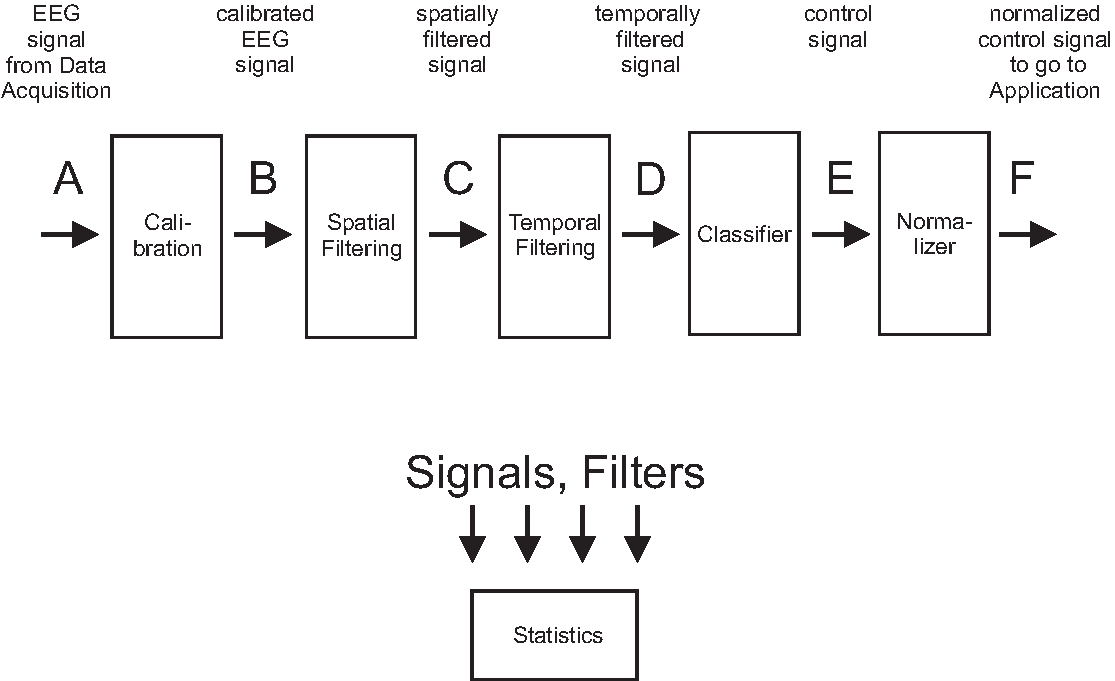
\includegraphics{figures/SigProcDataFlow}}}
 \caption{Data flow in the signal processing module}
 \label{sigprocdataflow}
\end{figure}

\subsection{Goals}

As described in chapter \ref{des_consid_goals}, one of the goals for this system 
is for each module to be as independent of the others as possible, e.g., Signal 
Processing should not have to take the type of data collection hardware into 
account. For the same reason, Application should (ideally) not have to know 
about the used signal processing method. While in real--world situations this 
will not be possible, control signals shall be normalized to the value range of 
short integers (-32767 to +32767), shall be zero mean (to the extent that this 
is possible), and each value shall be equally accessible by the user's EEG. In 
this fashion, the interdependence between Signal Processing and Application can 
be minimized.


\subsection{Assumptions and Dependencies}

Signal Processing can contain instances of multiple filter classes. These filter 
classes cannot assume any specific values for \textit{SampleBlockSize}, 
\textit{SamplingRate}, or \textit{TransmitCh}. They have to be able to adapt 
their functionality according to these three parameters -- they might not only 
be used in scenarios with varying parameters, but also they might have to work 
together with other filters. Therefore, hard coded assumptions about these three 
parameters have to be avoided.


\subsection{Module Initialization}

The GenericFilter's constructor requests parameters and states in the state 
vectors from the operator in the same fashion other classes (e.g., GenericADC) 
do. In order to distinguish different instances, the constructor can also be 
passed an integer defining the instance number. The constructor can ignore this 
instance number or it can request different parameters for each instance (e.g., 
WindowLength1 for instance 1, WindowLength2 for instance 2, etc.)


\subsection{Class Model}
\label{class_model}

Many classes in both Data Acquisition and Signal Processing are working on 
signals. Thus, we defined two similar classes: \textit{GenericSignal} (working 
with floating point numbers) and \textit{GenericIntSignal} (working with short integers).

\begin{verbatim}
class GenericSignal
{
private:
       int  *Elements;
public:
       GenericSignal(unsigned short NewChannels, int NewMaxElements);
       ~GenericSignal();
       float **Value;
       int   Channels;
       int   MaxElements;
       bool  SetElements(unsigned short Channel, int NewElements);
       int   GetElements(unsigned short Channel);
       bool  SetChannel(float *source, int channel);
       float *GetChannel(int channel);
       float GetValue(int Channel, int Element);
       bool  SetValue(int Channel, int Element, float Value);
};
\end{verbatim}


\begin{verbatim}
class GenericIntSignal
{
private:
       int  *Elements;
public:
       GenericIntSignal(unsigned short NewChannels, int NewMaxElements);
       ~GenericIntSignal();
       short **Value;
       int   Channels;
       int   MaxElements;
       bool  SetElements(unsigned short Channel, int NewElements);
       int   GetElements(unsigned short Channel);
       bool  SetChannel(short *source, int channel);
       short *GetChannel(int channel);
       short GetValue(int Channel, int Element);
       bool  SetValue(int Channel, int Element, short Value);
};
\end{verbatim}


The main class in Signal Processing besides the signal classes is the
class \textit{GenericFilter} and each filter class is derived from it.

\begin{verbatim}
class GenericFilter 
{
protected:
       STATEVECTOR       *statevector;
       TCustomWinSocket  *operatorsocket;
public:
       GenericFilter(PARAMLIST *ParamList, STATELIST *StateList);
       GenericFilter(PARAMLIST *ParamList, STATELIST *StateList, 
                     int instance);
       ~GenericFilter();
       int Initialize(PARAMLIST *ParamList, STATEVECTOR *statevector, 
                     TCustomWinSocket *opsocket);
       int Process(GenericSignal *Input, GenericSignal *Output);
};
\end{verbatim}


The class \textit{FILTERS} is a wrapper for all signals and filters in the 
SignalProcessing module. It instantiates and initializes each signal and filter, 
and for each incoming EEG signal block from Data Acquisition, its Process() 
method calls the Process() methods for each filter. This class is defined in the 
unit UFilterHandling.cpp -- \textbf{no other unit has to and should be touched, 
if you want to include your filter in the main program.}\footnote{
This is likely to change in the future such that copying and editing of framework code
can be avoided (which makes it difficult to maintain otherwise). If you implement
your filter's \texttt{Preflight()} member properly (see the error handling document
for details about this new member of \texttt{GenericFilter}), and if you add a
line \texttt{RegisterFilter(MyFilter, 2.x);} to your filter's cpp file,
you prepare for those changes.}

\begin{verbatim}
class FILTERS
{
protected:
       GenericSignal *CreateGenericSignal(int transmitchannels, 
                                          int samples, char *buf);
       int      numcontrolsignals, samples, transmitchannels;
public:
       FILTERS(PARAMLIST *ParamList, STATELIST *StateList);
       ~FILTERS();
       int      Initialize(PARAMLIST *plist, STATEVECTOR *svector, 
                           CORECOMM *corecomm);
       int      Process(char *buf);
       bool     error;
       CalibrationFilter  *calfilter;
       GenericSignal      *SignalA, *SignalAPrime, *SignalB;
       GenericSignal      *SignalC, *SignalD, *SignalDPrime;
};
\end{verbatim}


\subsection{Implementing Your Own Signal Processing Filter}

Integrating a new filter class into the system is simple:

\begin{enumerate}
 \item{Derive a class from \textit{GenericFilter} in a separate file}
 \item{Implement the constructor and the methods Initialize() and
       Process() (use the implementations in CalibrationFilter.cpp 
       as an example to start with and make sure that your methods
       have the same return values -- the main program depends on them)}
 \item{Include your new unit in the SignalProcessing project and include 
       its header file in UFilterHandling.h}
 \item{In UFilterHandling.h, add a pointer variable to your class to the class
       definition of FILTERS, e.g.,
       \begin{verbatim}CalibrationFilter  *calfilter;\end{verbatim}}  
 \item{In UFilterHandling.cpp, in the constructor of the FILTERS class,
       add code that instantiates your class, e.g., 
       \begin{verbatim}calfilter=new CalibrationFilter(plist, slist);\end{verbatim}}
 \item{In UFilterHandling.cpp, in the destructor of the FILTERS class,
       add code that deletes the instance of your class, e.g., 
       \begin{verbatim}if (calfilter) delete calfilter;\end{verbatim}}
 \item{In UFilterHandling.cpp, in the Initialize() method of the FILTERS class,
       add code that calls the Initialize() method of your filter, e.g., 
       \begin{verbatim}res=calfilter->Initialize(plist, svector, corecomm);\end{verbatim}}
 \item{In UFilterHandling.cpp, in the Process() method of the FILTERS class,
       add code that calls the Process() method of your filter, e.g., 
       \begin{verbatim}res=calfilter->Process(SignalA, SignalAPrime);\end{verbatim}}
\end{enumerate}


You might also want to add visualization capability to your filter. Currently, 
either the display of signals (channels x samples) or display of a memo field is 
supported. In addition, graphical output can be configured. Once again, this is 
pretty simple: 

\begin{verbatim} #include 
"UGenericVisualization.h"

 GenericVisualization *vis;

 // create an instance to GenericVisualization and pass
 // pointers to the parameterlist and the communication object
 vis= new GenericVisualization( paramlist, corecomm);

 // set the window title
 vis->SendCfg2Operator(SOURCEID_TEMPORALFILT, CFGID_WINDOWTITLE, "Temporal Filter");

 // set the number of samples to be displayed
 sprintf(cur_buf, "%d", nBins);
 vis->SendCfg2Operator(SOURCEID_TEMPORALFILT, CFGID_NUMSAMPLES, cur_buf);

 // set the minimum and maximum values in the graph
 vis->SendCfg2Operator(SOURCEID_TEMPORALFILT, CFGID_MINVALUE, "0");
 vis->SendCfg2Operator(SOURCEID_TEMPORALFILT, CFGID_MAXVALUE, "80");
 
 // specify the X axis labels for the graph
 for (i=0; i<nBins; i++)
  {
  sprintf(cur_buf, "%03d %.0f", i, (float)start+(float)i*(float)bandwidth);
  vis->SendCfg2Operator(SOURCEID_TEMPORALFILT, CFGID_XAXISLABEL, cur_buf);
  }

 // send out the signal to the Operator
 vis->Send2Operator(signal);   

 // another example; configure visualization as a memo and
 // send some ASCII text to the Operator:
 vis->SetSourceID(SOURCEID_TASKLOG);
 vis->SendCfg2Operator(SOURCEID_TASKLOG, CFGID_WINDOWTITLE, "User Task Log");
 sprintf(memotext, "Run: %d; ITI -> new trial: %d\r", run, trial);
 vis->SendMemo2Operator(memotext);
 
 delete vis;
\end{verbatim}

THAT'S IT !! After describing how to integrate a new filter into the system,
the following sections describe actual implementations of filter classes that
implement the respective filters in Figure \ref{sigprocdataflow}.

\subsection{Calibration}

The calibration filter (class \textit{CalibrationFilter}) calibrates the 
incoming EEG signal. It performs a linear scaling, such that each channel is 
expressed in $\mu$V and has a mean of zero (i.e., 
$\mathit{newvalue}=(\mathit{ADvalue}-\mathit{SourceChOffset})*\mathit{SourceChGain}$).

The calibration filter acts only on the subset of channels defined by
\textit{TransmitCh} and \textit{TransmitChList;} regardless of that, the
\textit{SourceChOffset} and \textit{SourceChGain} parameters
refer to the full set of software channels as stored in the data file, in
the order in which they are digitized.

\subsubsection{Requested Parameters}

\begin{table}[ht]
 \centering
 \begin{tabular}{|l|l|l|}
  \hline
  \textbf{Section} & \textbf{Parameter} & \textbf{Data Type}\\
  \hline
  Source & SourceChOffset & floatlist \\
  \hline
  Source & SourceChGain & floatlist \\
  \hline
  Source & AlignChannels & int \\
  \hline
 \end{tabular}
 \caption{Parameters requested by the class SpatialFilter}
\end{table} 

\textit{SourceChOffset} specifies a list of offsets in AD units -- one value
for each channel. \\
\textit{SourceChGain} specifies a list of gains as used in described formula -- 
one value for each channel. \\
\textit{AlignChannels} specifies, whether samples should be aligned in time --
most data acquisition boards multiplex one A/D converter and thus samples
for \textit{SoftwareCh} channels are linearly distributed in time over 
$\frac{1000}{SamplingRate}$ milliseconds (0=no alignment, 1=perform alignment).

\subsubsection{Input/Output}

The input to an instance of this filter class is GenericIntSignal A (dimensions 
\textit{TransmitCh} channels by \textit{SampleBlockSize} elements). Its output 
is Signal B with the same dimensions.


\subsection{Spatial Filter}

The spatial filter class \textit{SpatialFilter} performs for each sample vector 
(\textit{TransmitCh} values -- one for each channel) an operation as shown in 
Figure \ref{spat_filt_op}.

\begin{figure}[ht]
 \centerline{\scalebox{1.0}{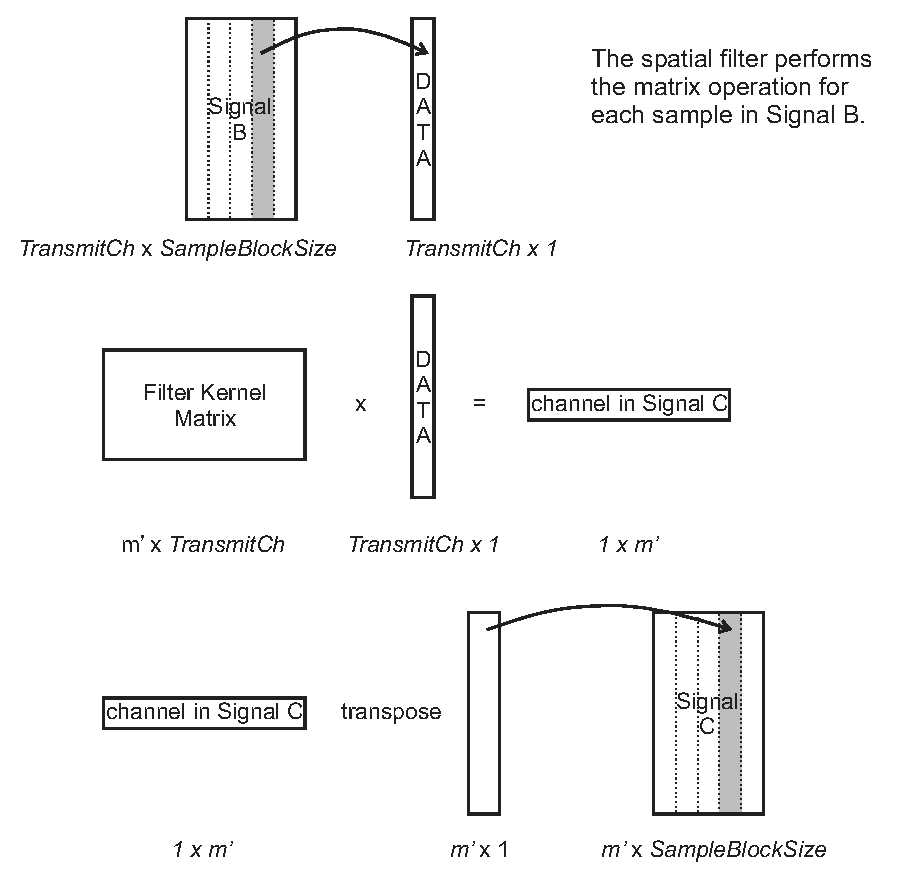
\includegraphics{figures/SpatFiltMatOp}}}
 \caption{Matrix operation on the input signal}
 \label{spat_filt_op}
\end{figure}


\subsubsection{Requested Parameters}

\begin{table}[ht]
 \centering
 \begin{tabular}{|l|l|l|}
  \hline
  \textbf{Section} & \textbf{Parameter} & \textbf{Data Type}\\
  \hline
  Filtering & SpatialFilterKernel & matrix \\
  \hline
 \end{tabular}
 \caption{Parameters requested by the class SpatialFilter}
\end{table} 

The dimensions of \textit{SpatialFilterKernel} are \textit{m'} by 
\textit{TransmitCh}.

\subsubsection{Input/Output}

The input to an instance of this filter class is Signal B (dimensions 
\textit{TransmitCh} channels by \textit{SampleBlockSize} elements). Its output 
is Signal C with the following dimensions: \textit{m'} channels and 
\textit{SampleBlockSize} elements.


\subsection{Temporal Filter Using an AR Model}

Each instance of the temporal filter class \textit{ARFilter} requests 
the following parameters:

\subsubsection{Requested Parameters}

\begin{table}[ht]
 \centering
 \begin{tabular}{|l|l|l|}
  \hline
  \textbf{Section} & \textbf{Parameter} & \textbf{Data Type}\\
  \hline
  Filtering & TempFiltCfg & matrix \\
  \hline
 \end{tabular}
 \caption{Parameters requested by the class ARFilter}
\end{table} 

\textit{TempFiltCfg} is a matrix of dimensionality m' x (max nr. of columns). It
serves to configure the nature of temporal filtering. \\


\subsubsection{Input/Output}

The input to an instance of this filter class is Signal C (dimensions number of 
spatially filtered channels by \textit{SampleBlockSize} elements). Its output is 
Signal D with the following dimensions: m' x n'.



\subsection{Classifier / Translation Algorithm}

An instance of \textit{ClassifierFilter} transforms pre--processed signal 
components into signals that can -- after normalization -- be used for device 
control.

\subsubsection{Requested Parameters}

\begin{table}[ht]
 \centering
 \begin{tabular}{|l|l|l|}
  \hline
  \textbf{Section} & \textbf{Parameter} & \textbf{Data Type}\\
  \hline
  Filtering & MUD & matrix \\
  \hline
  Filtering & MLR & matrix \\
  \hline
 \end{tabular}
 \caption{Parameters requested by the class ClassifierFilter}
\end{table} 

\textit{MUD} and \textit{MLR} are matrices of the same dimensionality as Signal 
D (m' x n'). The two scalars in the resulting control signal (Signal E) -- one 
for up/down and one for left/right movement -- each are linear combinations of 
Signal D and their respective weight matrix (\textit{MUD} or \textit{MLR}) as 
follows: $updown=\sum_{i=0,j=0}^{i<m',j<n'}{MUD_{ij}*SignalD_{ij}}$


\subsubsection{Input/Output}

The input to this filter class is Signal D with the following dimensions: m' x 
n'. The output is Signal E with \textit{NumControlSignals} channels and 1 
element per channel.


\subsection{Normalizer}

An instance of \textit{NormalizeFilter} makes each scalar in the vector of
control signals (Signal E) zero mean and thereafter normalizes it to a 
desired range (not exceeding -32767 to +32767).

\subsubsection{Requested Parameters}

\begin{table}[ht]
 \centering
 \begin{tabular}{|l|l|l|}
  \hline
  \textbf{Section} & \textbf{Parameter} & \textbf{Data Type}\\
  \hline
  Filtering & Gain & floatlist \\
  \hline
  Filtering & Intercept & floatlist \\
  \hline
 \end{tabular}
 \caption{Parameters requested by the class NormalizeFilter}
\end{table} 

Each of the \textit{NumControlSignals} scalars in \textit{Gain} and 
\textit{Intercept} are used as follows: 
$SignalF_{i}=Gain_{i}*(SignalE_{i}+Intercept_{i})$


\subsubsection{Input/Output}

The input to this filter class is Signal E with the following dimensions: 
\textit{NumControlSignals} channels and 1 element per channel. Its output,
Signal F, is of the same dimensionality.


%Example of instantiating a Signal:

%\begin{verbatim}
%GenericSignal *SignalA;
%SignalA = new GenericSignal(TransmitCh, SampleBlockSize);
%for (unsigned short n=0; n<TransmitCh; n++) 
%    SignalA->SetElements(n, SampleBlockSize);
 
%The program flow is:

%CreateFilters();
%SendParameters();
%GetParameters();
%Initialize();

%While( active )
%{	
%Receive( A, StateVector );									
%SpatialFilter( A, B );
%TemporalFilter( B, C );
%Classifier( C, D );
%Send( D, StateVector );
%Statistics( A, B, C, D );
%}
%\end{verbatim}

%CreateFilters() Instantiates each filter object.  The constructor of each filter 
%object fills up the parameter list with AddParameter( *parameterlist ) and 
%requests any state fields with AddState( *statelist ).  SendParameters() 
%publishes this list to the operator.  GetParameters() receives the parameter 
%list from the operator. Initialize() instantiates the GenericSignal objects, 
%parameterizes the signal processing routines, and creates a global state 
%vector..

%Each of the Filter modules calls the entire list of filters of its type as below:

%\begin{verbatim}
%Signal SpatialFilter(GenericSignal A, GenericSignal B)
%{
% Laplacian( A, B );
% Car( A , B);
% Null( A , B);
%}
%\end{verbatim}

%The signals A, B, C and D are not requested parameters because they are always 
%present in the signal processing module. For each of the signal processing 
%methods the recipe (e.g. B= f( A ) is in the parameters requested by that 
%method.  The method goes through it's k copies of it's parameters and computes 
%the signals indicated in each set of parameters. Any filter can send 
%visualization data to the operator.  This has implications for concurrency 
%control.


\subsection{Slow-Wave-Feedback}

\subsubsection{Author and Introduction}

Description of Signal Processing Module for the Slow-Wave-Feedback written by 
Thilo Hinterberger, University of Tuebingen, Germany.

The calculation of the Slow-Wave feedback signal is subdivided into three 
modules: The SW-Filter, which is realized as an efficient boxcar-filter, the 
SetBaseline module, which subtracts a defined baseline from the signal and an 
artifact correction module, which contains two different artifact correction 
modes.  

\begin{figure}[ht]
 \centerline{\scalebox{0.8}{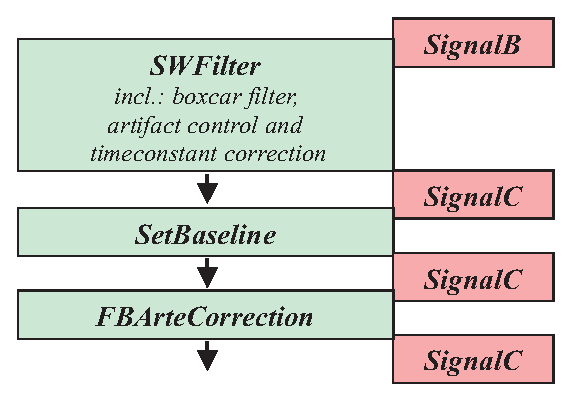
\includegraphics{figures/SWFilterFlow}}}
 \caption{Data flow in the slow wave filter}
 \label{swfilterdataflow}
\end{figure}

\subsubsection{Temporal SW-Filter}

Following states are used:
Artifact (bool) is set to 1 when the signal changes exceed the threshold values defined in ThresholdAmp (see below).  
BeginOfTrial is checked to trigger the start of the trial and reset the internal counter.

\subsubsection{Requested Parameters}

The SW-Filter uses the following parameters:

\begin{verbatim}
SWFilter int SWAvgSpan= 0.5 0.5 0 10 
         // Averaging window in s
SWFilter intlist SWInChList= 3 0 1 2 0 0 63 
         // Channel index of input signal (include artifact channel!)
SWFilter intlist SWOutChList= 3 0 1 2 0 0 63 
         // Channel index of output signal (include artifact channel!)
SWFilter floatlist ThresholdAmp= 3 100 100 400 200 -2000 2000 
         // Threshold for invalid Trial in uV
SWFilter float Tc= 0 16 0 1024 
         // Time constant filter settings in s
Visualize int VisualizeSWFiltering= 1 0 0 1  
          // visualize SW filtered signals (0=no 1=yes)
\end{verbatim}

SWAvgSpan defines the time window of the boxcar-filter. SWInChList defines, 
which channels from Signal B are filtered. They are sorted to the channels in 
Signal C which are selected in SWOutChList. In the Standard setting, three 
channels are filtered. The ThresholdAmp is an artifact control parameter. In 
between one trial (from one BeginOfTrial to the next), the amplitude is not 
allowed to vary more than the in ThresholdAmp defined size in �V. Otherwise the 
trial should be neglected and set as invalid in the application module (state 
Artifact is set to one). A time constant (Tc) correction function simulates a 
real DC-behaviour, even if the amplifier has no DC-option. This can be done by 
the knowledge of the amplifiers' time constant, which is set as the parameter 
Tc. To avoid that the signal will drift towards very high positive or negative 
values, the correction signal is set to zero each time, when BeginOfTrial is 
one. Tc=0 will switch off the Tc-correction. Note: The Tc-correction will only 
work properly, when the A/D-converter and the amplifier puts out 0 when the 
input is 0 �V and there is no electrode polarization! If you are not sure, 
switch off this correction.

\subsubsection{Baseline Setting}

Following states are used:
Baseline (bool) is set to 1 during the baseline period between BaseBegin and BaseEnd. Otherwise it is zero.
BeginOfTrial is checked to trigger the start of the trial and reset the internal counter.

\subsubsection{Requested Parameters}

The SW-Filter uses the following parameters:

\begin{verbatim}
BLFilter float BaseBegin= 0.9 1.9 0 60 
         // Begin of Baseline in s
BLFilter float BaseEnd= 1.0 2.0 0 60 
         // End of Baseline in s
BLFilter intlist BaseChList= 3 1 1 1 1 0 1 
         // 1 to mark that BL is subtracted
Visualize int VisualizeBaselineFiltering= 1 0 0 1  
          // visualize baseline filtered signals (0=no 1=yes)
\end{verbatim}

The baseline is set each trial at the time point BaseEnd seconds after 
BeginOfTrial was set to one. The baseline amplitude is the average amplitude in 
the time interval between BaseBegin and BaseEnd. The baseline is subtracted of 
all channels marked with 1 in the BaseChList. As default, baseline subtraction 
is applied on all three channels.

This version still uses the parameters BIPts and FIPts, which define the 
duration of the baseline-interval and the feedback-interval in seconds. These 
parameters are used for the buffer, which needs the duration of a trial. They 
will be no longer used in the next version.  

\subsubsection{Artifact Correction}

Following states are used:

Artifact (bool) is set to 1 only in ArteMode=3 when the feedback signal is set 
to zero due to the EOG artifact BeginOfTrial is checked to trigger the start of 
the trial and reset the internal counter.

\subsubsection{Requested Parameters}

The SW-Filter uses the following parameters:

\begin{verbatim}
ArteFilter intlist ArteChList= 3 2 2 -1 2 -1 63
  // Assignment of artefact channels, -1: no artifact channel
ArteFilter floatlist ArteFactorList= 7 0.15 0.15 0 0 0 0 0 0 -1 1
  // Influence of artefact channel on input channel,
     -1: no artifact channel
ArteFilter int ArteMode= 0 1 0 3
  // Artefact correction mode, 0 off, 1 continuous, 2 conditioned
Visualize int VisualizeFBArteCorFiltering= 1 0 0 1 
  // visualize FBArte corrected signals (0=no 1=yes)
\end{verbatim}

Artifacts are corrected on all channels which are not marked with -1
in the ArteChList. For the correction, the channel number at the
position of the channel in the ArteChList is used as artifact channel.
For example, the standard setting corrects the channels 0 and 1 by using
channel 2 for the correction. The correction factor is the factor set
in ArteFactorList, 0.15 in the standard setting.

For the ArteMode parameter, the following values are possible: 
\begin{itemize}
 \item\verb|ArteMode 0| switches this filter off.
 \item\verb|ArteMode 1| will subtract the artifact channel multiplied 
      with a constant factor.
 \item\verb|ArteMode 2| will correct the signal according to Koutchoubey, 1997:
      If the artifact's absolute value does not exceed that of the control signal,
      the control signal is corrected by subtracting the artifact signal; otherwise,
      feedback is suppressed.
%\begin{verbatim}
%     if ((ArteSignal*ControlSignal) > 0) {            // if they have same signs
%        if (fabs(ArteSignal) < fabs(ControlSignal)) InputSignal->Value[m][n] = ControlSignal-ArteSignal;  // if Artefact not too big then correct
%        else {                             // artifact is too big
%            InputSignal->Value[m][n] = 0;  // FB is supressed
%            if (ArteMode==3) statevector->SetStateValue("Artifact",1);
%        }
%     }
%\end{verbatim}
 \item\verb|ArteMode 3| is working identically to \verb|ArteMode 2| but sets the
      Artifact state to 1 when the feedback is set to zero.
\end{itemize}


\section{User Application}


\subsection{General Information}

As described in chapter \ref{goals_module_independence}, one major goal for 
system design is the independence between modules. In most BCI systems, however, 
some parts of the signal processing applied (i.e., the device-dependent part of 
signal processing) depend on the feedback to the user -- a feature provided by 
the user application.

This inter-dependence between signal processing and the user application poses 
severe problems to the system design, because it is not possible to completely 
encapsulate each module and separate it from others.

In order to minimize inter-dependence, duties should be performed by the module
that is conceptually defining it, e.g., task paradigm and timing are conceptually
parts of a task and should therefore be handled by the user application module.

Section \ref{section_rjb_task} describes a particular implementation of a user
task - a simple cursor task - that complies with this motivation.


\subsection{Right Justified Box Task}
\label{section_rjb_task}

The right justified box task is a cursor task, in which the subject tries to hit 
one out of \textit{n} targets on a screen in trials of equal length. As listed 
in 
%table \ref{blablabla} and
figure \ref{rjb_task}, the task requests and 
controls specific states.

Whatever signal processing algorithm is used, it can passively monitor these 
states and modify its operation accordingly, e.g., one algorithm might derive 
its baseline from the inter-trial interval (i.e., ITI), whereas another might 
calculate it differently. In this fashion, signal processing algorithms can be 
interchanged without affecting the user application.

\begin{figure}[ht]
 \centerline{\scalebox{0.6}{\includegraphics{figures/RJBtask}}}
 \caption{Time Line for Right Justified Box task. The top-most target position
          corresponds to TargetCode=1. TargetCode increases towards the bottom.
          ResultCode corresponds to the target actually selected. Thus, if
          TargetCode equals ResultCode, the trial was a hit, otherwise a miss.}
 \label{rjb_task}
\end{figure}

Figure \ref{rjb_task} illustrates the time line for the right justified box task 
and, for each time interval, its respective content for each state. 

1 is the intertrial interval, were the screen is blank and baseline data can be 
collected (optional). In 2 the target is presented, but the cursor is absent (no 
feedback).  In 3 the cursor is present and it's vertical movement is controlled 
by the user's EEG.  Horizontal cursor movement is under computer control and is 
at a constant rate.  In 4 the cursor approaches the target and in 5 the target 
has been hit and trial-outcome feedback is presented.  In 6 the screen is blank 
(intertrial interval again) and in 7 another target is presented.

\section{Entity--Relationship Model for Shared Classes}

\begin{figure}[ht]
 \centerline{\scalebox{0.9}{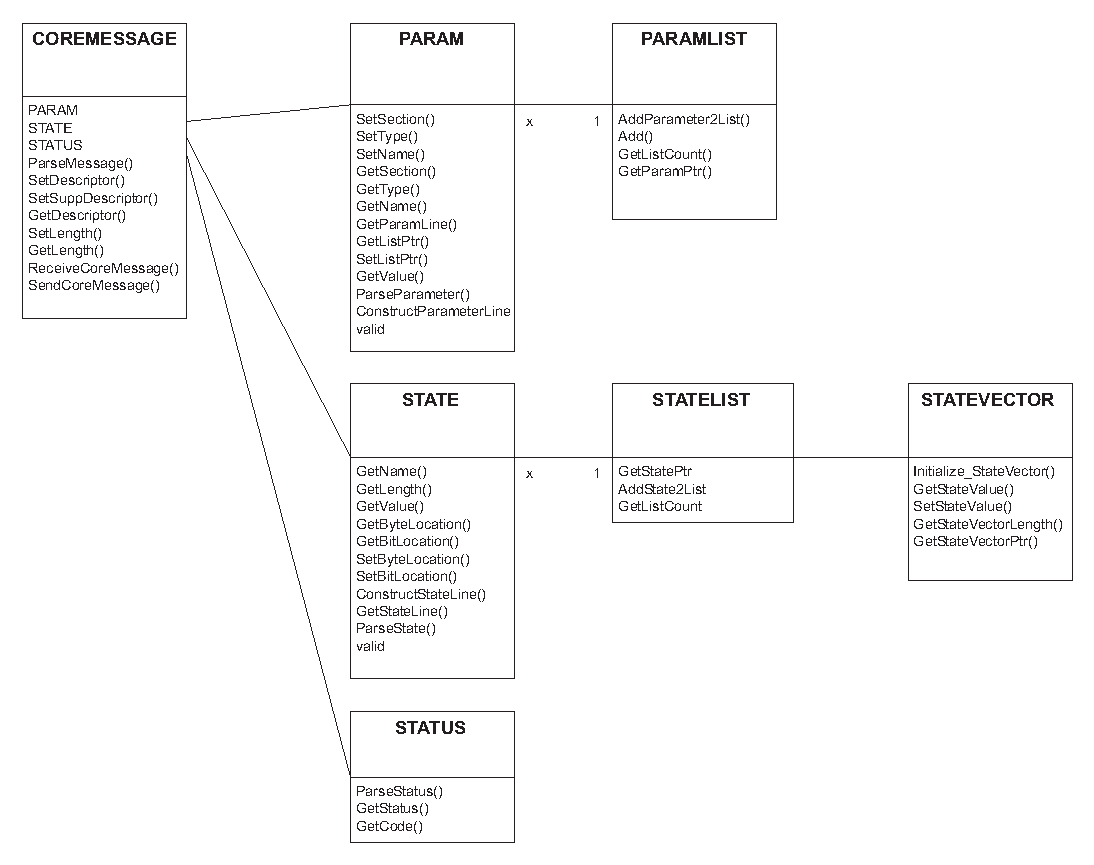
\includegraphics{figures/ERmodel_shells}}}
 \caption{Class model for all shared classes}
\end{figure}


%Most components described in the System Architecture section will require a more 
%detailed discussion. Other lower-level components and subcomponents may need to 
%be described as well. Each subsection of this section will refer to or contain a 
%detailed description of a system software component. The discussion provided 
%should cover the following software component attributes: 

%Classification 

%The kind of component, such as a subsystem, module, class, package, function, 
%file, etc. .... 

%Definition 

%The specific purpose and semantic meaning of the component. This may need to 
%refer back to the requirements specification. 

%Responsibilities 

%The primary responsibilities and/or behavior of this component. What does this 
%component accomplish? What roles does it play? What kinds of services does it 
%provide to its clients? For some components, this may need to refer back to the 
%requirements specification. 

%Constraints 

%Any relevant assumptions, limitations, or constraints for this component. This 
%should include constraints on timing, storage, or component state, and might 
%include rules for interacting with this component (encompassing preconditions, 
%postconditions, invariants, other constraints on input or output values and 
%local or global values, data formats and data access, synchronization, 
%exceptions, etc.) 


%Composition 

%A description of the use and meaning of the subcomponents that are a part of 
%this component. 


%Uses/Interactions 

%A description of this components collaborations with other components. What 
%other components is this entity used by? What other components does this entity 
%use (this would include any side-effects this entity might have on other parts 
%of the system)? This concerns the method of interaction as well as the 
%interaction itself. Object-oriented designs should include a description of any 
%known or anticipated subclasses, superclasses, and metaclasses. 

%Resources 

%A description of any and all resources that are managed, affected, or needed by 
%this entity. Resources are entities external to the design such as memory, 
%processors, printers, databases, or a software library. This should include a 
%discussion of any possible race conditions and/or deadlock situations, and how 
%they might be resolved. 


%Processing 

%A description of precisely how this components goes about performing the duties 
%necessary to fulfill its responsibilities. This should encompass a description 
%of any algorithms used; changes of state; relevant time or space complexity; 
%concurrency; methods of creation, initialization, and cleanup; and handling of 
%exceptional conditions. 

%Interface/Exports 

%The set of services (resources, data, types, constants, subroutines, and 
%exceptions) that are provided by this component. The precise definition or 
%declaration of each such element should be present, along with comments or 
%annotations describing the meanings of values, parameters, etc. .... For each 
%service element described, include (or provide a reference) in its discussion a 
%description of its important software component attributes (Classification, 
%Definition, Responsibilities, Constraints, Composition, Uses, Resources, 
%Processing, and Interface). 

%Much of the information that appears in this section is not necessarily expected 
%to be kept separate from the source code. In fact, much of the information can 
%be gleaned from the source itself (especially if it is adequately commented). 
%This section should not copy or reproduce information that can be easily 
%obtained from reading the source code (this would be an unwanted and unnecessary 
%duplication of effort and would be very difficult to keep up-to-date). It is 
%recommended that most of this information be contained in the source (with 
%appropriate comments for each component, subsystem, module, and subroutine). 
%Hence, it is expected that this section will largely consist of references to or 
%excerpts of annotated diagrams and source code. Any referenced diagrams or 
%source code excerpts should be provided at any design reviews. 